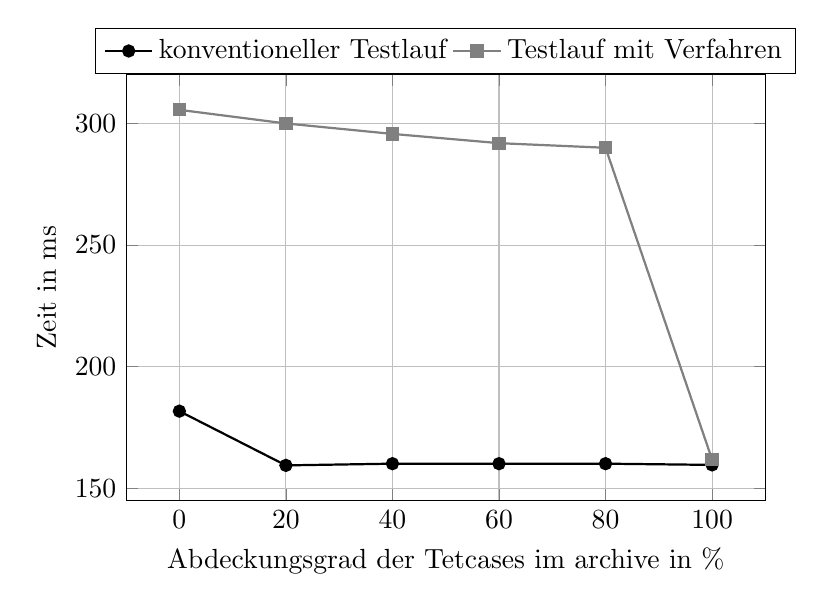
\begin{tikzpicture}
    \begin{axis}[
        width=0.8\textwidth,
        height=7cm,
        xlabel={Abdeckungsgrad der Tetcases im archive in \%},
        ylabel={Zeit in ms},
        grid=major,
        legend style={
            at={(0.5,1.0)},
            anchor=south,
            legend columns=2
        }
    ]
    \addplot[
        thick,
        mark=*,
    ] coordinates {
        (0, 181.7)
        (20, 159.4)
        (40, 160.1)
        (60, 160.1)
        (80, 160.1)
        (100, 159.6)
    };
    \addlegendentry{konventioneller Testlauf}
    \addplot[
        thick,
        mark=square*,
        gray!100,
    ] coordinates {
        (0, 305.6)
        (20, 300)
        (40, 295.7)
        (60, 291.9)
        (80, 290.0)
        (100, 161.8)
    };
    \addlegendentry{Testlauf mit Verfahren}
    \end{axis}
\end{tikzpicture}
